\label{sec:XPS}\index{XPS} XPS is a tool to achieve information of the samples chemical structure.
Most of the information given here is taken from \cite{Riviere_90} in \cite{briggs_auger_1990}.
If X-rays hit metals electrons can be emitted. This effect is called photoelectric effect and was first discovered by Heinrich Hertz in 1887 throught the fact that electrodes illuminated with ultraviolet light create electric sparks more easily\cite{hertz_ueber_1887}. 18 years later Albert Einstein received the Nobel Price for his discovery of the law of the photoelectric effect\cite{_nobel_2015} and a scientific explanation for this effect which Hertz was missing.

\paragraph{physics behind XPS}
As the X-rays hit and penetrate the sample surface they excite electrons and initiate several different processes:
\begin{itemize}
 \item core level and valence level electron excitation
 \item auger electron excitation(p. 91 in \cite{Briggs_90})
\end{itemize}
\label{XPS}
For the \textbf{simple core-level excitation} the X-ray removes a single electron next to the core which is then detected. Energy conservation due to elastic scattering of the electron out of the bulk results in the relation 
\begin{align}
E_{kin} &= h\nu_{\textnormal{X-ray}}-E_{B}-\Phi_{\textnormal{bulk}} \\
E_B 	&=h\nu_{\textnormal{X-ray}}-E_{kin}-\Phi_{\textnormal{bulk}}
\end{align}
 $h\nu_{\textnormal{X-ray}}$ is the energy of the incident X-ray beam, $E_B$ the binding energy of the excited electron and $\Phi_{bulk}$ the work function of the analyser. 
 
The standard X-ray source is supplied with aluminium and magnesium anodes. Other materials are available that produce various X-ray energies and line widths \index{XPS!Anode materials} \cite{_x-ray_2015}. 
\begin{table}\caption{Energy and line widths of available anode materials. Taken from }
 \centering
 \begin{tabular}{cccc}
Anode 	& 	Radiation 	& Photon Energy (eV) 	& Line Width (eV) \\
Mg	&	K$\alpha$ 	&	1253.6	&	0.7\\
Al	&	K$\alpha$ 	&	1486.6 	&	0.85\\
Zr 	&	L$\alpha$ 	&	2042.4 	&	1.6\\
Ag 	&	L$\alpha$ 	&	2984.3 	&	2.6\\
Ti 	&	K$\alpha$ 	&	4510.9 	&	2.0\\
Cr	&	K$\alpha$ 	&	5417 	&	2.1\\
 \end{tabular}
\end{table}

 In the \textbf{Auger process} \index{XPS!Auger process} on the other hand the created core level (lets say at level K) vacancy is filled with a energetically higher lying electron (at for example level $L_1$). The excess energy can either be radiated away (X-ray fluorescence) or given to an electron in the same or in a more shallow level (lets say $L_{2,3}$). This electron then can leave the sample as Auger electron. Figure \ref{fig:auger-core} shows the mentioned process. 
 
 Due to the fact that this process has two stages these electrons are referred to as secondary electrons. The notation for this process is $KL_1L_{2,3}$. The electron taking part in the Auger process can also originate from within the valence band ($KL_{2,3}V$) or even both electrons may stem from the valence band ($KVV$). For every element there is a unique series of Auger excitations. This holds even if one or even both electrons come from a valence band, as the dominating term will always be the binding energy $E_K$. As the Auger energy $$E_{KL_1L_{2,3}}=E_K-E_{L_1}-E_{L_{2,3}}$$ is not a function of the excitation energy it will not shift when changing the X-ray energy. Even very heavy elements (as the number of atomic levels the possible Auger transitions profiliate) do not exhibit a very large number of Auger emission lines due to the fact that the transition propability favourates only a few of this many. \cite{Briggs_90}

\begin{figure}\centering
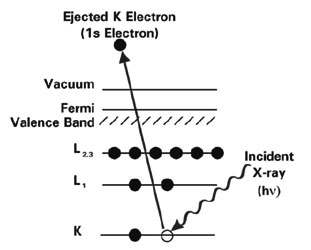
\includegraphics[height=0.3\textwidth]{./images/whatisxps-04.jpg}
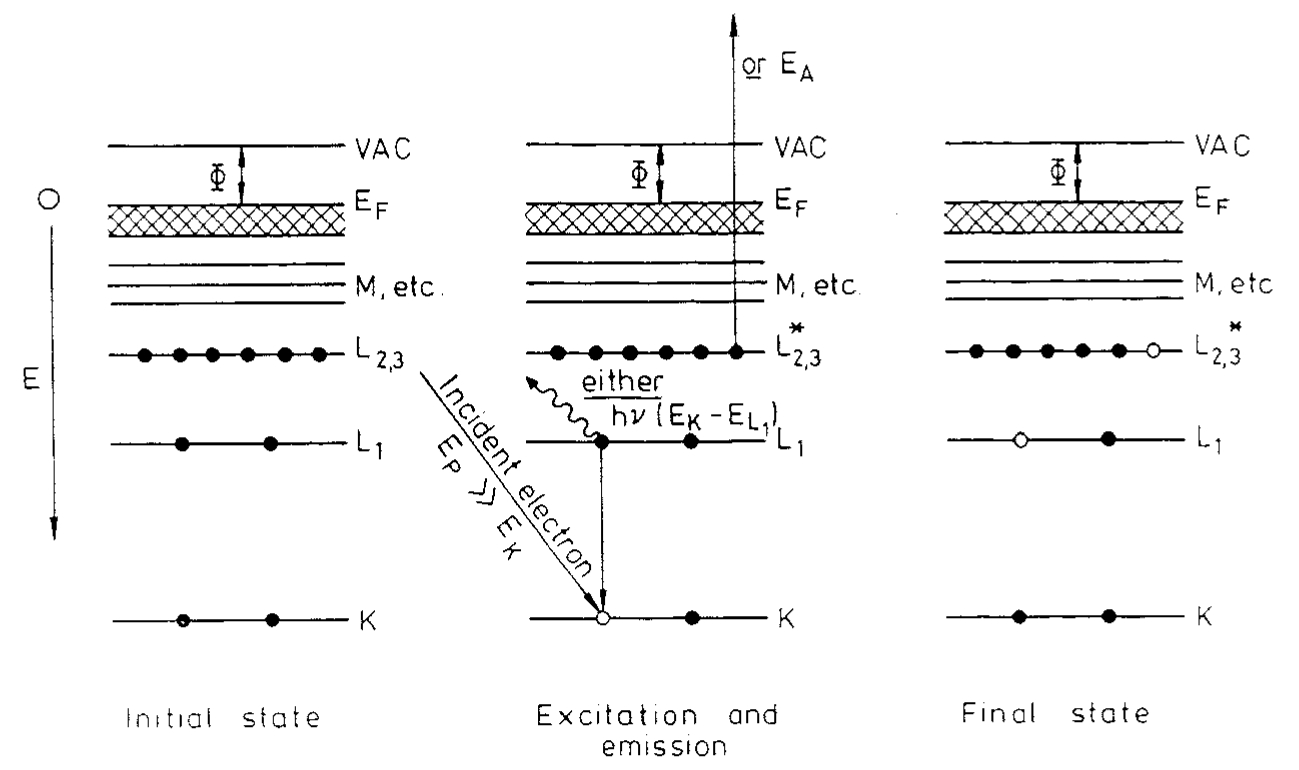
\includegraphics[height=0.45\textwidth]{./images/auger.jpg}
\caption{Shematic diagram of the process of Auger emission in a solid. Taken from \cite{_whatisxps-04.jpg_2015}(left/obove) \cite{Briggs_90}(right/lower)}
\label{fig:auger-core}
\end{figure}

The \index{XPS!chemical surrounding} chemical surrounding of atoms changes their binding energy, making XPS an ideal tool to detect changes in chemial surrounding. Although the analysis is averaged over the area of the incident X-rays (typically hundrets of mircons up to several mm) its results are very precise. This makes it possible to distinguish differently bound atoms within single atomic species and therefore gives rise to otherwise not directly observable processes like growth, intercalation, etching and binding of for example graphene islands on Ir(111)\cite{busse_graphene_2011-1,granas_oxygen_2012}.

With the use of aluminium X-ray sources, electrons are excellerated with typically \SI{15}{\keV} onto the targets. Most of the created radiation goes into the principal characteristic line ($K\alpha_{1,2}$). Higher ones ($K\alpha_{3,4}$, $K\beta$) are also observed but with much lower intensities. In addition there is a continuous background called Bremsstrahlung extending up to the energy of the incident electron energy. This background is of no use for the XPS measurement and has to be substtracted in a more or less artificial way.

For the ease of analysis, many spectra are recorded with monochromatized radiation. This selects a certain energy for the following illumination of the sample. This technique relies on the dispersion of X-rays within a crystal. It is described by the Bragg relation $n\lambda = 2d\sin(\theta)$ where n is the diffraction order, $\lambda$ the wavelength of monochromatized radiation, d the distance between two crystal layers and $\theta$ is the so called Bragg angle. The first order peak for Al $K\alpha$ radiation ($\lambda=\SI{0,83}{\nm}$, $E=\SI{1486,6}{\eV}$) is at $\theta=\SI{78.5}{\degree}$ (using the $10\bar10$ planes of a quartz crystal with $d=\SI{0,425}{\nm}$). Therefore the angle between incident and reflected beam is about \SI{23}{\degree}.\cite{Riviere_90}

The spectra used in this work are recorded without monochromatized radiation as not stated otherwise.

The \index{XPS!binding energies} binding energies of some often observed peaks are given in table \ref{tab:XPS-intensities}
\begin{table}\centering
 \caption{Position and origin of several XPS peaks, taken from\cite{wanger_handbook_1979}}
 \begin{tabular}{llll}
  Eelement & excited state & Binding energy [eV]& comment\\ \hline \hline
  O & 1s & 531&\\
  N & 1s & 398,1&\\
  C & 1s & 285&\\
  B & 1s & 189,4& \\
  Cu & 2p & 953 (1/2), 933 (3/2) & suitable for oxidation analysis\\
  Cu & LMM & 560-580 & suitable for oxidation analysis\\
  Cu & 3s & 123 &\\
  Cu & 3p & 77 (1/2), 75 (3/2) & \\
 \end{tabular}
\label{tab:XPS-intensities}
\end{table}
% \begin{figure}
% 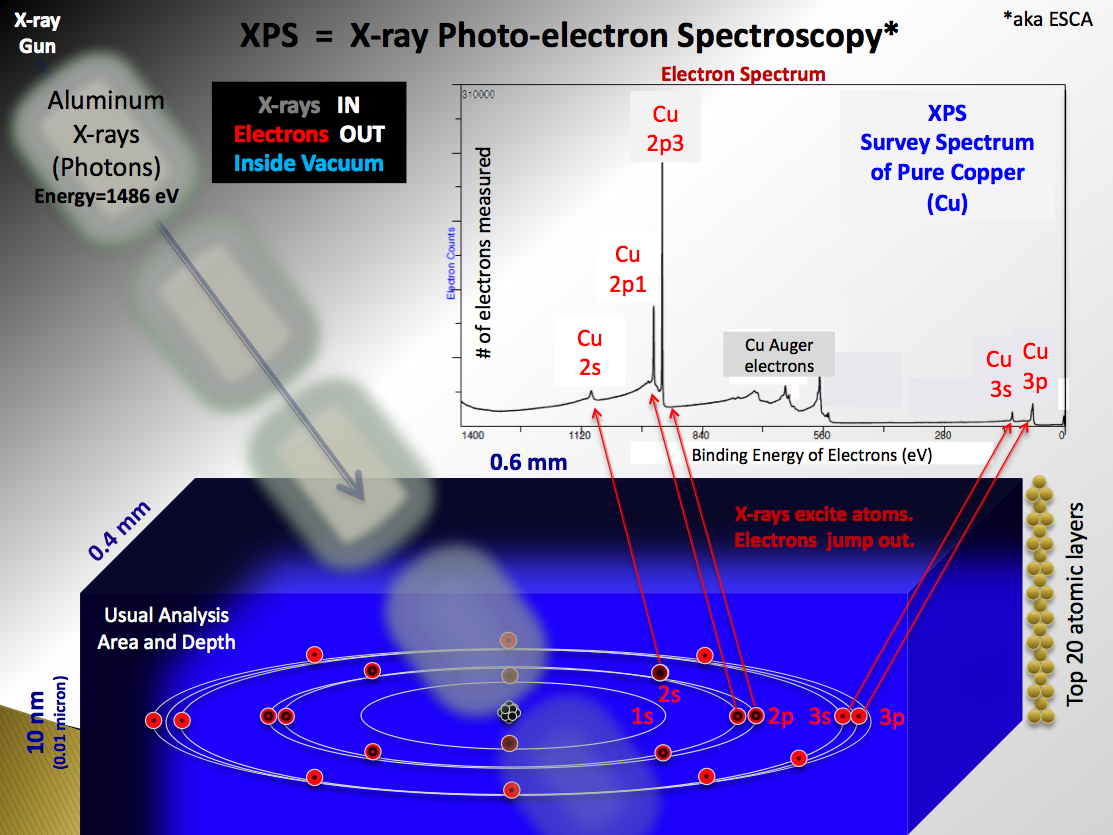
\includegraphics[width=0.7\textwidth]{./images/XPS_PHYSICS.jpg}
% \caption{Sketch of the XPS process. Taken from \cite{_xps_physics.png_2015}}
% \end{figure}
\paragraph{Peak shapes}\index{XPS!Peak shapes}
The shape of the peaks typically resembles the line shape of the used Xrays (Gauss width $\approx 1eV$). In case of s-states (l=0) (B1s, N1s, C1s) the peaks are singulets. With increasing j=l+s, the spin-orbit (j-j) coupling introduces a 'parallel' and 'anti-parallel' nature of the spin, resulting in two different j=1/2(3/2) and therefore two different energies. The split in energy is expected to increase as Z increases (for constant n,l) or as l decreases (n constant). This makes the splitting of 3p orbitals larger than that of the 3d's. The ratio of the two peaks is given by their degeneracy (2j+1).\cite[113]{Riviere_90}
\begin{table}
\caption{Spin-orbit splitting parameters. Reproduced from \cite{Riviere_90}}
\centering
 \begin{tabular}{ccc}
 Subshell & j values & Area ratio \\
 s & $\frac{1}{2}$ & --- \\
 p & $\frac{1}{2}$,$\frac{3}{2}$ & 1:2 \\
 d & $\frac{3}{2}$,$\frac{5}{2}$ & 2:3 \\
 f & $\frac{5}{2}$,$\frac{7}{2}$ & 3:4 \\
 \end{tabular}
\end{table}


\paragraph{experimental setup}
As discussed above, the XPS setup requieres a source of X-ray, an monochromator (optional) and an electron detector that can scan the energy range up to the X-ray energy. The detector selects the energy to be recorded via a \underline{\ \ \ \ \ \ \ \ \ \ \ \ }.
\paragraph{quantitative analysis}
The more atoms of a specific kind are present, the larger the signal gets. Therefore the signal intensity resembles the amount of atoms on the topmost surface layers($\approx \SI{10}{\nm}$).

As each irridiated atomic species has a different cross section for adsorption of X-rays with a certain energy they emit auger and core level spectra with a different intensity. Comparing the cross section of e.g. N with B's, one can see that it it roughly 3-4 times as large (B: \SI{6,87e3}{\barn\per atom}, N: \SI{25,82e3}{\barn\per atom} for $\textnormal{Al} K_{\alpha}$)\cite{henke_x-ray_1993}. Meaning that the signal from the N is much stronger than that of the B, although their number of atoms is equal.

A calibrated XPS is capable of measuring the surface coverage of an adlayer (e.g. BN) compared to the bulk of the sample. Calibration works as follows:
\begin{itemize}
 \item A perfect, full layer of a known material (e.g. C) is prepared (graphene)
 \item The known cross section for C (\SI{6,87e3}{\barn\per atom})\cite{henke_x-ray_1993} relates the signal to the number of atoms of the full layer.
 \item One only has to devide the signal of the unknown coverage (of known material) by the cross section (of C) and directly receives the coverage. Keep in mind that the X-ray penetration depth (and with it the signal of the substrate) stays only constant if the illumination angle stays constant. Even small angular variations may change the signal.
\end{itemize}
Refering to \cite{ertl_low_1986} the fraction $\theta_A$ of an adsorbate A on a surface B can be calculated via
\begin{equation}\label{eq:adlayer-coverage}
 \theta_A=\frac{I_AI_B^0\cdot \exp(\frac{a_A}{\lambda_A}\cos(\Theta))}{I_AI_B^0(\cdot \exp(\frac{a_A}{\lambda_A}\cos(\Theta))-1)+I_BI_A^0\cdot \exp(\frac{a_A}{\lambda_A}\cos(\Theta))}
\end{equation}
where 
\begin{table}[h!]\centering
\caption{Description of parameters used in equation \ref{eq:adlayer-coverage}}
 \begin{tabular}{cc}
  Parameter & Annotation \\ \hline \hline
  $I_A$	& integrated intensity of the adsorbate peak \\
  $I_A^0$ & cross section of element A \\
  $\lambda_A$ & mean free path of electrons in material A \\
  $a_A$ & thickness of adlayer \\
 \end{tabular}
\end{table}
The mean free path of electrons with energy E in a solid is given by $\lambda_M=\SI{0,41}{}\cdot a_M^{\SI{0,41}{}}\cdot E_M^{\SI{0,5}{}} $ where $a_M$ is the atomic size of M. 

Literature:
\begin{itemize}
 \item Photoabsorption cross sections for various elements \cite{henke_x-ray_1993})
  \item oxidation processes of Cu: \cite{deroubaix_x-ray_1992}.
\end{itemize}